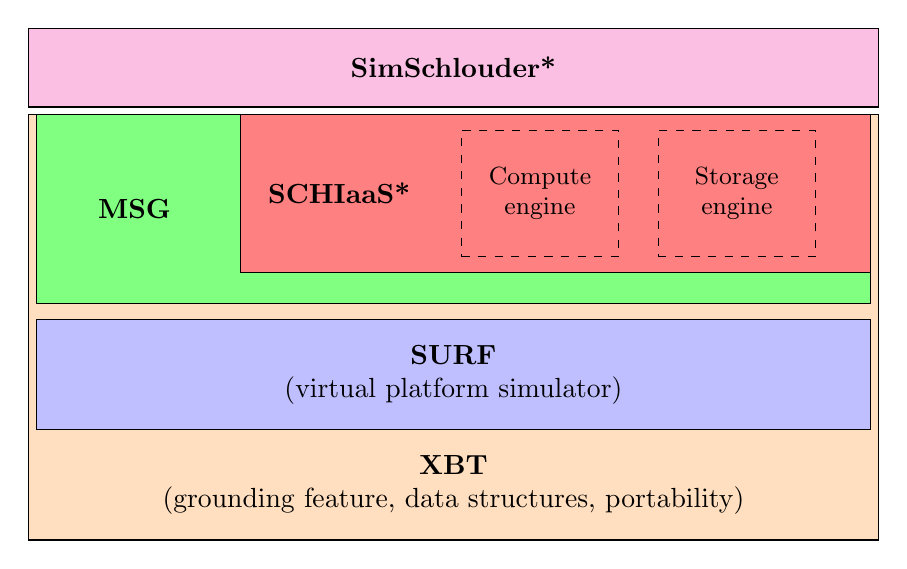
\begin{tikzpicture}[x=1cm,y=1cm,
every node/.style={
rectangle,
align = center,
anchor=south west,
outer sep=1mm,
},
box/.style={
draw,
}]

%Simgrid box
\node[box,minimum height=5.4cm,minimum width=10.8cm,fill=orange!25,
%label={south:\small{}\textsf{\textbf{SimGrid}}}
]at(0,0){};
%\node[box,minimum height=5.8cm,minimum width=1.4cm,fill=cyan!50]at(11,0){\rotatebox{270}{\textbf{Tracing}}};
\node[minimum height=1.4cm,minimum width=10.6cm]at(0.1,0){\textbf{XBT}\\(grounding feature, data structures, portability)};
\node[box,minimum height=1.4cm,minimum width=10.6cm,fill=blue!25]at(0.1,1.4){\textbf{SURF}\\(virtual platform simulator)};
\node[box,minimum height=2.4cm,minimum width=10.6cm,fill=green!50]at(0.1,3){};
\node[minimum height=2.4cm,minimum width=2.5cm]at(0.1,3){\textbf{MSG}};
\node[box,fill=red!50,minimum height=2cm,minimum width=8cm]at(2.7,3.4){};
\node[minimum height=2cm,minimum width=2.5cm]at(2.7,3.4){\textbf{SCHIaaS*}};
\node[box,dashed,minimum height=1.6cm,minimum width=2cm]at(5.5,3.6){};
\node[anchor=center,font=\small]at(6.6,4.5){Compute\\engine};
\node[box,dashed,minimum height=1.6cm,minimum width=2cm]at(8,3.6){};
\node[anchor=center,font=\small]at(9.1,4.5){Storage\\engine};
\node[box,fill=magenta!25,minimum width=10.8cm,minimum height=1cm]at(0,5.5){\textbf{SimSchlouder*}};
\end{tikzpicture}